\documentclass[journal]{IEEEtran}
\usepackage[utf8]{inputenc}
\usepackage{cite}
\usepackage{amsmath,amssymb,amsfonts}
\usepackage{graphicx}
\usepackage{textcomp}
\usepackage{xcolor}
\usepackage{stfloats}
\usepackage{booktabs}
\usepackage{tabularx}
\usepackage{microtype}
\usepackage{balance}
\usepackage{xurl}
\usepackage[hidelinks]{hyperref}

\setcounter{topnumber}{4}
\setcounter{bottomnumber}{4}
\setcounter{totalnumber}{10}
\setcounter{dbltopnumber}{4}
\renewcommand{\topfraction}{0.95}
\renewcommand{\bottomfraction}{0.95}
\renewcommand{\textfraction}{0.05}
\renewcommand{\floatpagefraction}{0.85}
\renewcommand{\dbltopfraction}{0.95}
\renewcommand{\dblfloatpagefraction}{0.85}

\ifdefined\pdfcompresslevel
\pdfcompresslevel=9
\fi
\ifdefined\pdfimageresolution
\pdfimageresolution=600
\fi

\def\BibTeX{{\rm B\kern-.05em{\sc i\kern-.025em b}\kern-.08em
T\kern-.1667em\lower.7ex\hbox{E}\kern-.125emX}}

\begin{document}

\title{Genuine Price Anomaly Detection and Q-Learning Dispatch for Battery Storage}

\author{Keshav~Aggarwal,~\IEEEmembership{Member,~IEEE,}
Mukesh~Singh,~\IEEEmembership{Senior~Member,~IEEE,}
Ashima~Singh,~\IEEEmembership{Senior~Member,~IEEE,}
Wayes~Tushar,~\IEEEmembership{Senior~Member,~IEEE,}
and~Arnab~Bhattacharjee,~\IEEEmembership{Senior~Member,~IEEE}%
\thanks{K. Aggarwal, M. Singh, and A. Singh are with the Electrical and Instrumentation Engineering Department, Thapar Institute of Engineering and Technology, Patiala 147004, India (e-mail: kaggarwal3\_be24@thapar.edu; msingh@thapar.edu; ashima@thapar.edu).}%
\thanks{W. Tushar is with the School of Information Technology and Electrical Engineering, The University of Queensland, Brisbane, QLD 4072, Australia (e-mail: w.tushar@uq.edu.au).}%
\thanks{A. Bhattacharjee is with the School of Engineering, Newcastle University, Newcastle upon Tyne, NE1 7RU, U.K. (e-mail: arnab.bhattacharjee@newcastle.ac.uk).}%
}

\maketitle

\begin{abstract}
\bfseries
Battery energy storage systems (BESS) in peer-to-peer (P2P) electricity markets capture the majority of their annual profits during rare, high-magnitude price spikes.
Conventional anomaly detection filters used for markets tend to regard valid price hikes as errors or attacks and limit battery discharge, losing out on large arbitrage gains within an hour.
This paper proposes a framework that combines unsupervised deep recurrent autoencoders with reinforcement-learning-based dispatch and can be directly deployed in existing battery controllers. 
First, a gated recurrent unit (GRU) autoencoder evaluates 24-hour rolling market prices to spot scarcity peaks, followed by a tabular Q-learning controller that schedules battery storage and releases energy when prices reach their peak.
Unlike conventional benchmarks that assume future price clairvoyance, the proposed causal framework enforces strict real-time execution. Evaluated on four years of authentic California Independent System Operator (CAISO) Day-Ahead settlements across three regional hubs (SP15, NP15, ZP26), the GRU detector achieves an Area Under the Receiver Operating Characteristic Curve (AUROC) of 0.882.
Conditioning tabular Q-learning on this anomaly alert quadruples energy trading profits while reducing cross-seed policy variance by 90\%, and the defense filter recovers up to 71.6\% of adversarial attack damage while comfortably exceeding the break-even threshold (76.5\% vs.\ 61.1\%).
These results demonstrate that wholesale price excursions represent high-value dispatch opportunities rather than telemetry corruptions, maximizing storage profitability within existing market-clearing rules.\end{abstract}


\begin{IEEEkeywords}
\bfseries
Adversarial robustness, anomaly detection, battery energy storage systems, California Independent System Operator, energy arbitrage, locational marginal prices, reinforcement learning, tabular Q-learning.
\end{IEEEkeywords}

\section{Introduction \& Literature Review}
\label{sec:intro}

Electricity prices in California have grown considerably more unpredictable in recent years. Solar output during the afternoon sun usually pushes locational marginal prices (LMPs) down toward zero, and sometimes below it, only for prices to snap back once the sun sets and fossil-fuel peaker generation dispatches at higher marginal costs to cover the evening peak. Battery Energy Storage Systems (BESS) exploit this daily rhythm in decentralized power grids and peer-to-peer (P2P) trading frameworks to charge their systems when power is cheap and discharge as prices climb~\cite{Chen_DRL_BESS, P2P_Systems_Book}.

Most days, these curves follow a common pattern dictated by the work schedule and the weather. However, a battery's annual profits tend to depend on a handful of extreme hours. Hourly prices can soar over \$1,000/MWh during heatwaves, transmission outages, and sudden generator trips, and a 10 MW / 10 MWh battery that fully discharges just once during such a spike can profit about as much as it would have made in a whole week otherwise. It is therefore a high priority for storage operators to detect these rare hours as soon as possible and to anticipate them. 

Past state-of-the-art (SOTA) approaches to anomaly detection in pricing have addressed the problem primarily from a cybersecurity perspective~\cite{Vulnerability_Analysis, AE_Anomaly, Xie_FDI}. Such an approach starts by using historical data without anomalies, creates some artificial price spikes, and checks whether the added anomalies are detected. Such an approach may be useful in defending against a cyber-attack~\cite{Kurt_FDI_Detection}. However, it cannot prove the actual trading process, the origins of prices, or the legal procedures governing market settlements. If a legitimate \$1,000/MWh spike anomaly is detected and battery discharge is disabled, the operator will incur significant income loss.

Thus, to explain the reason for our experimental evaluations, we use only actual market prices, obtaining settlement information from the California Independent System Operator (CAISO) Open Access Same-Time Information System (OASIS) website~\cite{CAISO} without any synthetic additions. We also investigate common questions, such as: Does the attacker actually inject fake spikes into this data flow, and how can storage assets defend against such tampering?

Using historical market data has two crucial issues. The first is that the historical prices provided by market operators cannot be taken as ground-truth labels; therefore, the model needs to be validated for statistical consistency and, ultimately, profitability. The second and even more important issue is that mistakes are not symmetrical in any sense. While a mistake in image or text recognition is just an annoyance, a mistake that prevents the battery from discharging into a real \$1,000/MWh spike can lead to a loss.

This work sits at the intersection of electricity price forecasting~\cite{Lago_EPF_Benchmark}, unsupervised time-series anomaly detection~\cite{AE_Anomaly, Audibert_USAD}, generative modeling~\cite{VAE, DDPM}, P2P energy trading~\cite{Chen_DRL_BESS, P2P_Systems_Book}, and battery dispatch optimization~\cite{RL_Dispatch, Shi_BESS_Coopt, He_CAISO_BESS, Sutton_RL}.

Electricity Prices and Anomaly Detection:
Rolling statistics, moving averages, and local z-scores are traditional approaches for detecting abnormal price levels in SOTA models. Although these are one of the simplest approaches to apply, they have limitations: they assume constant thresholds that do not change with the seasons; a threshold set in winter to accommodate low load levels will always result in alarms in summer.

The deep models learn the usual 24-hour price pattern directly from historical data; there are no predefined patterns in our models. The recurrent autoencoders (Long Short-Term Memory (LSTM), Gated Recurrent Unit (GRU)) propagate sequence states forward in time, compress each daily path into a small bottleneck, and detect the moments when reconstruction error becomes large~\cite{Audibert_USAD}. On the other hand, the variational autoencoders (VAEs) encode price windows into a continuous latent space~\cite{VAE}, and the denoising diffusion probabilistic models (DDPMs) add Gaussian noise to the input and learn to remove this process~\cite{DDPM}. Large price spikes are unusual, making it harder to remove noise and leading to frequent, large errors.

Battery Dispatch and Trading: Storage scheduling, commonly used methods include model predictive control (MPC), linear programming, and dynamic programming~\cite{Shi_BESS_Coopt}, while reinforcement learning (RL) is increasingly seen as an alternative to these methods~\cite{RL_Dispatch, Chen_DRL_BESS, Sutton_RL}. One of the flaws frequently found in benchmarks reported in the literature is an implicit assumption of precognition about tomorrow's prices; when the optimizer is aware of the prices in advance, then there is no need for anomaly detection at all. This problem is avoided by ensuring that every dispatch instance is performed in a purely causal manner.

The reasons behind these two problems, lack of labeled data and imbalanced misclassification costs, inspire the design choices made in this paper. The paper has contributions in the following aspects:
\begin{itemize}
\item Performance analysis of various anomaly detection architecture models using iForest (Isolation Forest), VAE, denoising diffusion, single-node LSTM and GRU, multi-variate LSTM, and Graph Attention Network on 28,271 market hours worth of CAISO settlement data (extended from 2023 to 2026 with an increase in data up to 32,832 market hours) through five random seeds and two separate testing intervals.
\item Dispatch policies spanning rules-based, directional, and RL methods to understand how controllers exploit anomaly signals, demonstrating that tabular Q-learning achieves maximum exploitation of the detection signal.
\item Analysis of economic break-even point accuracy ($p^*$) evaluates the feasibility of defense mechanisms in terms of asymmetric risk.
\end{itemize}

\section{Mathematical Modeling}
\label{sec:math_model}

The physical storage restrictions, detection criteria, RL dynamics, and adversarial risk are defined formally using notation and operational parameters presented in Table~\ref{tab:nomenclature}.

\begin{table}[!t]
\centering
\caption{Nomenclature and Parameter Settings}
\label{tab:nomenclature}
\footnotesize
\renewcommand{\arraystretch}{1.15}
\begin{tabularx}{\columnwidth}{l>{\raggedright\arraybackslash}X}
\toprule
\textbf{Symbol} & \textbf{Description} \\
\midrule
$s_t$ & Anomaly score for the 24h window ending at hour $t$ \\
$H$ & Window length ($H = 24$\,hours) \\
$x_{t,h}, \hat{x}_{t,h}$ & Normalized observed and reconstructed price at hour $h$ \\
$Q(s, a)$ & Action-value estimate for state $s$ and action $a$ \\
$\alpha, \gamma$ & Q-learning rate ($\alpha=0.15$) and discount factor ($\gamma=0.95$) \\
$r_t$ & Net arbitrage cash return at hour $t$ (\$) \\
$E_t$ & Battery stored energy level at hour $t$ ($0 \le E_t \le 10$\,MWh) \\
$SoC_t$ & State-of-charge ratio ($SoC_t = E_t / C \in [0, 1]$) \\
$C, P_{\max}$ & Rated energy capacity (10\,MWh) and power limit (10\,MW) \\
$e, \Delta t$ & Round-trip cycle efficiency ($e=0.80$) and interval ($\Delta t=1$\,h) \\
$c_{\text{fee}}, c_{\text{deg}}$ & Market fee (\$0.50/MWh) and cell degradation (\$2.50/MWh) \\
\bottomrule
\end{tabularx}
\end{table}

Dynamics of discrete-time energy storage characterize the physical behavior of the BESS.:
\begin{equation}
E_{t+1} = E_t + \left( \eta_{\text{ch}} P_t^{\text{ch}} - \frac{1}{\eta_{\text{dis}}} P_t^{\text{dis}} \right) \Delta t,
\label{eq:soc_dynamics}
\end{equation}
subject to the constraints of operability, storage capacity, and exclusivity:
\begin{align}
0 \le P_t^{\text{ch}} \le P_{\max}, \quad 0 \le P_t^{\text{dis}} \le P_{\max}, \label{eq:p_limits} \\
0 \le E_t \le C, \quad P_t^{\text{ch}} \cdot P_t^{\text{dis}} = 0, \label{eq:soc_limits}
\end{align}
where $P_t^{\text{ch}}$ and $P_t^{\text{dis}}$ denote charge and discharge power at hour $t$, respectively, with $P_{\max} = 10$\,MW, $C = 10$\,MWh, and $\Delta t = 1$\,h. Symmetric one-way conversion efficiencies satisfy $\eta_{\text{ch}} = \eta_{\text{dis}} = \sqrt{e} = \sqrt{0.80} \approx 0.894$, guaranteeing a round-trip cycle efficiency of $e = \eta_{\text{ch}}\eta_{\text{dis}} = 0.80$. The state-of-charge ratio is defined as $SoC_t = E_t / C \in [0, 1]$.

\begin{figure*}[!t]
\centering
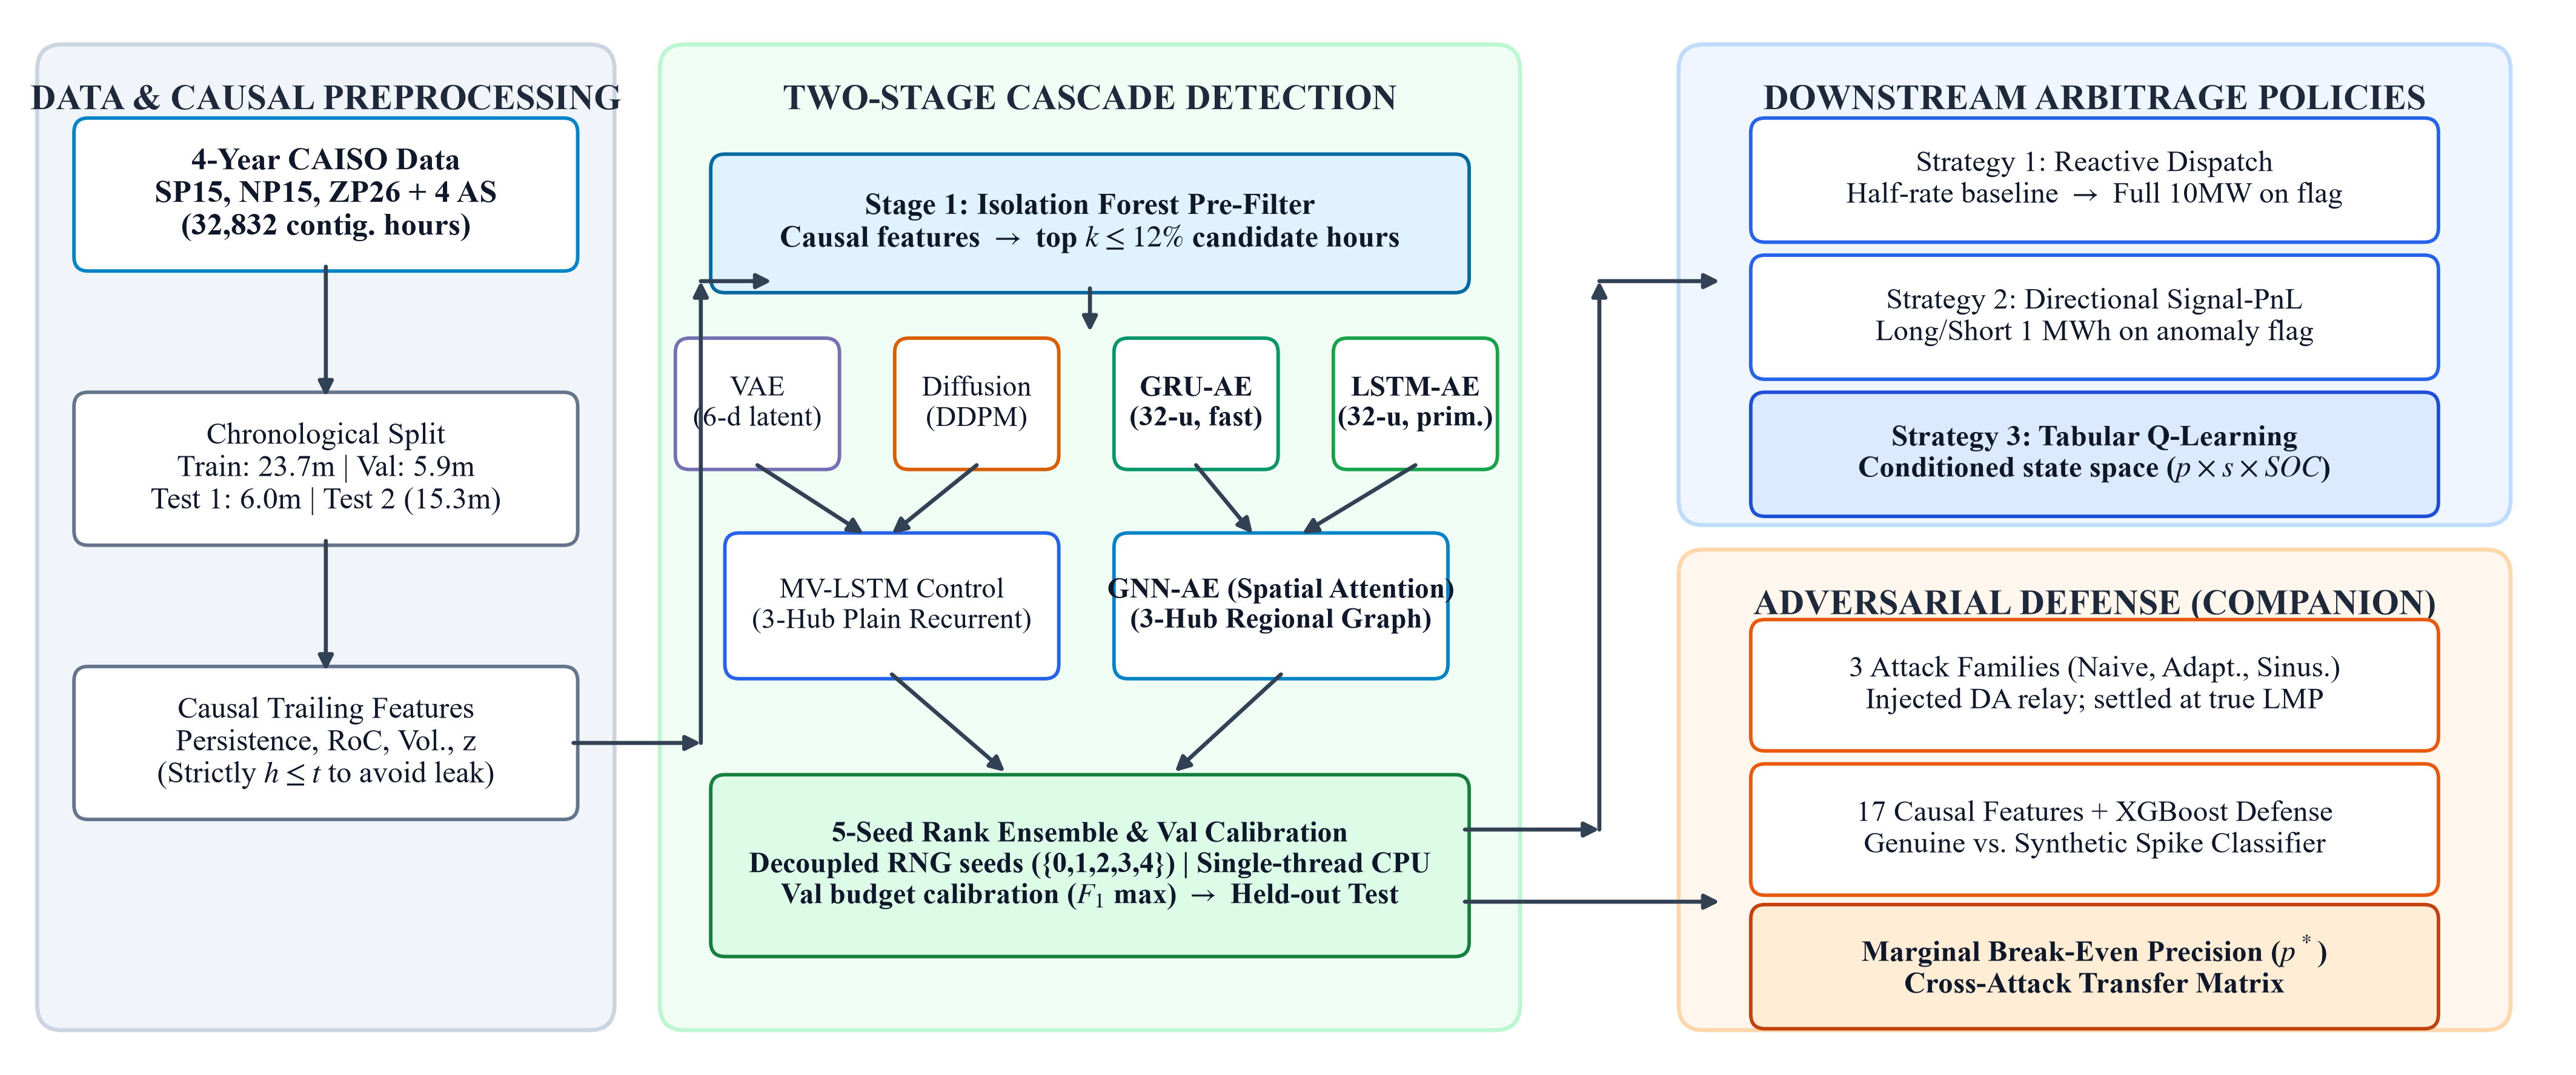
\includegraphics[width=0.96\textwidth]{architecture.png}
\caption{System architecture. The raw CAISO price data undergoes causal feature extraction before Stage 1, which consists of an iForest pre-filter, followed by Stage 2, which consists of deep autoencoders and multi-node models. The five-seed ensemble then guides the battery dispatching policy and the defense filter.}
\label{fig:architecture}
\end{figure*}

Deep autoencoders analyze normalized 24-hour causal price time series and calculate anomaly scores using the mean square reconstruction error:
\begin{equation}
s_t = \frac{1}{H}\sum_{h=1}^{H}\left(x_{t,h}-\hat{x}_{t,h}\right)^2.
\label{eq:score}
\end{equation}
Usually, the autoencoder successfully reconstructs the price graph for the particular day. However, when prices increase suddenly, the compressed representation cannot encode the change, and $s_t$ increases sharply.

In the case of GNN-AE, the transmission topology graph $\mathcal{G} = (\mathcal{V}, \mathcal{E})$ is specified for the three California hubs as $\mathcal{V} = \{\text{NP15}, \text{ZP26}, \text{SP15}\}$ where the set of edges $\mathcal{E}$ is the transmission links for Path 15 (NP15-ZP26) and Path 26 (ZP26-SP15). The two graph attention layers calculate the spatial direction attention coefficients $\alpha_{ij}$:
\begin{equation}
\alpha_{ij} = \frac{\exp\left(\text{LeakyReLU}\left(\mathbf{a}^T [\mathbf{W} h_i \parallel \mathbf{W} h_j]\right)\right)}{\sum_{k \in \mathcal{N}_i} \exp\left(\text{LeakyReLU}\left(\mathbf{a}^T [\mathbf{W} h_i \parallel \mathbf{W} h_k]\right)\right)},
\label{eq:gat}
\end{equation}
where $\mathbf{W} \in \mathbb{R}^{8 \times d}$ is a shared projection matrix ($d=24$), $\mathbf{a} \in \mathbb{R}^{16}$ is the attention vector, $\parallel$ denotes concatenation, and $\mathcal{N}_i$ represents adjacent regional hubs. Spatial node representations feed into an LSTM temporal sequence encoder.

The Tabular Q-Learning~\cite{Sutton_RL} uses as its finite state space $s = (p_z, a_{\text{flag}}, s_{\text{soc}})$. Prices are normalized and discretized in 10 buckets with boundaries ranging between $-3\sigma -  +3\sigma$ (price level buckets are $p_z \in \{1, \dots, 10\}$); the anomaly flag value $a_{\text{flag}}$ belongs to 5 quantiles of severity ($a_{\text{flag}} \in \{1, \dots, 5\}$; or $1$ class in unconditional baseline) while the SoC value bucket range is also $s_{\text{soc}} \in \{1, \dots, 5\}$. It gives $|S|=250$ discrete states ($|S|=50$ in conditional absence of anomaly).

The action space comprises of three discrete values for power commands $a \in \{-1.0, 0.0, 1.0\}$, indicating full battery discharge ($P_t^{\text{dis}}=P_{\max}$), resting ($P_t=0$), and full battery charging ($P_t^{\text{ch}}=P_{\max}$), satisfying \eqref{eq:soc_dynamics}-\eqref{eq:soc_limits}. The exclusive nature of actions is implied by the discrete set of actions. The net return for rewards for money received $r_t$ includes:
\begin{align}
r_t ={}& \left( p_t P_t^{\text{dis}} - p_t P_t^{\text{ch}} \right) \Delta t \nonumber \\
&- \left[ c_{\text{fee}} \left( P_t^{\text{dis}} + P_t^{\text{ch}} \right) + c_{\text{deg}} P_t^{\text{dis}} \right] \Delta t,
\label{eq:reward}
\end{align}
where cell degradation $c_{\text{deg}}$ is linearized per discharged MWh equivalent following~\cite{Xu_BESS_Degradation}. Action values are updated iteratively via:
\begin{equation}
Q(s,a) \leftarrow Q(s,a) + \alpha \left[r_t + \gamma \max_{a'} Q(s',a') - Q(s,a)\right],
\label{eq:qlearning}
\end{equation}
with learning rate $\alpha=0.15$ and discount factor $\gamma=0.95$.

\section{Methodology}
\label{sec:methodology}

Approximately 4 years of hourly day-ahead LMPs from CAISO are investigated, including data from 12th January, 2023, to 11th October, 2026. The price information was collected at the three main prosumer aggregation points, namely, SP15, NP15, and ZP26, and four ancillary services, Regulation Up, Regulation Down, Spinning Reserves, and Non-Spinning Reserves, amounting to 28,271 price observations in a 24-hour period (32,832 for continuous grid time-indexed hours). The latter are used as background information for multi-channel anomalies, representing the reserve margin tightness of the system operation. At the same time, only energy arbitrage calculations are evaluated in economic trading terms.

In addition to that, price anomalies have been observed during the above-mentioned period where SP15 recorded its highest at $\$1,143.78/ \text{MWh}$ on 17th August, 2023, owing to heat waves in the region, whereas its lowest was on 19th May, 2024, where SP15 recorded a price of $-\$41.33/ \text{MWh}.$

To give a more pragmatic estimate on the efficiency of our method, we divide time into non-overlapping intervals as follows: training interval from 12th January, 2023 to 31st December, 2024 (17,280 consecutive hours, about 23.7 months), validation interval from 1st January to 30th June, 2025 (4,344 hours, 5.9 months: solely for the calibration of the thresholds), and testing interval from 1st July, 2025 to 11th October, 2026 (11,208 hours, 15.3 months: tested once). Moreover, the six-month out-of-season seasonality test period is from 1st January to 30th June in 2025. In the case of California electric markets, the clearing of the Day-Ahead Market (DAM) takes place for all 24 hours of the next day of operation at 13:00 $D-1$. Nevertheless, BESS commercial traders and transactive prosumers must place their bids for energy deliveries without knowing the settled prices before 10:00 AM. They must roll their exposures to real-time imbalances on a 15-minute and 5-minute basis. We test our models using only causal 24-hour rolling windows in order to eliminate the problem of foreseeing.

As no native anomaly labels were available from historical settlement prices, the ex-post benchmarking flag was constructed purely for reference purposes – an hour gets flagged if its settlement price deviates by more than 4 median absolute deviations (MAD) from the 30-day moving median or lies within the tail 0.5\% of the distribution (this happened 739 times out of 28,271 hours, $\sim$2.6\%). The intervals flagged in this manner correlate perfectly well with confirmed CAISO reserve capacity scarcity periods, such as Heatwave Flex Alerts and severe evening net-load ramps. None of the models was provided with the flag data in any way during the training procedure. Most importantly, to avoid circular assessment, the effectiveness of the detection system is not judged on the sole basis of statistical labels but in terms of the physical trading surplus of the market (Section~\ref{sec:results}). Sensitivity analysis confirms that model family rankings remain invariant across MAD thresholds from 3.0 to 5.0.

The detection architecture (Fig.~\ref{fig:architecture}) employs a two-stage pipeline: Stage 1 iForest screens coarse outliers, followed by Stage 2 deep sequence models for refined scoring.

Stage 1 iForest~\cite{IForest} uses nine causal features: (i) trailing 6-hour linear slope $\Delta p / \Delta t$, (ii) non-reversion ratio $|p_t - p_{t-1}| / (|p_{t-1} - p_{t-2}| + \epsilon)$, (iii) 1-hour difference $(p_t - p_{t-1})$, (iv) 3-hour difference $(p_t - p_{t-3})$, (v) 24-hour robust $z$-score $(p_t - \text{median}_{24}) / \text{MAD}_{24}$, (vi) 168-hour trailing $z$-score, (vii) 24-hour rolling volatility $\sigma_{24}$, and (viii--ix) cyclic diurnal harmonics $(\sin(2\pi h / 24), \cos(2\pi h / 24))$.

A total of three models have been implemented for Stage 2 single-node detection. VAE has been trained for 40 epochs with the Adam optimizer ($\text{lr}=10^{-3}$, batch size=64). The VAE architecture consists of fully connected networks with 48 neurons, and the bottleneck is modeled as an 8-dimensional Gaussian distribution~\cite{VAE}. LSTM-AE and GRU-AE map the price sequence through 32 recurrent neurons to an 8-dimensional bottleneck.

The neural network is trained using the Adam optimization algorithm, with a learning rate of $10^{-3}$, a batch size of 32, and 40 training epochs. The training uses the mean squared error loss function~\cite{Audibert_USAD}. In the GRU case, the update and reset gates are used, which makes training 25\% faster but does not affect temporal dependencies. The DDPM learns how to reverse the procedure of adding noise to the data on discrete schedules~\cite{DDPM}. The inference step involves corrupting the window samples at four noise levels ($t \in \{0.10, 0.25, 0.40, 0.60\}$) over 16 iterations and averaging the residuals.

To explore the influence of the regional transmission environment on predictability, we also use SP15, NP15, and ZP26 as inputs to two multi-hub models: a 3-channel multi-variate LSTM (MV-LSTM) control and the GNN-AE~\cite{GAT}.

All experiments were executed across five random seeds (0--4) with fixed CPU thread allocation (\texttt{torch.set\_num\_threads(1)}) and deterministic seeds. All experiments were performed on an Intel Core i7-1355U platform (10 cores, up to 5.0\, GHz boost, 16\, GB RAM, 512\, GB NVMe SSD) under Windows 11. Code was developed using \texttt{numpy} (v2.0+), \texttt{pandas} (v2.2+), \texttt{scipy} (v1.14+), \texttt{scikit-learn} (v1.5+), \texttt{torch} (v2.4+), \texttt{xgboost} (v2.0+), and \texttt{matplotlib} (v3.8+).

\begin{table*}[!t]
\centering
\caption{Performance Master Summary: Accuracy of Model Reconstruction and Anomaly Identification}
\label{tab:detector_results}
\footnotesize
\renewcommand{\arraystretch}{1.2}
\setlength{\tabcolsep}{3.5pt}
\begin{tabular*}{\textwidth}{@{\extracolsep{\fill}}lccccccccc@{}}
\toprule
& \multicolumn{2}{c}{\textbf{Reconstruction Error ($\downarrow$)}} & \multicolumn{4}{c}{\textbf{Anomaly Detection Accuracy ($\uparrow$)}} & \multicolumn{3}{c}{\textbf{Operating Point Metrics ($\uparrow$)}} \\
\cmidrule(lr){2-3} \cmidrule(lr){4-7} \cmidrule(lr){8-10}
\textbf{Model Architecture} & \textbf{RMSE (\$)} & \textbf{MAE (\$)} & \shortstack{\textbf{Mean}\\\textbf{AUROC}} & \shortstack{\textbf{Ens.}\\\textbf{AUROC}} & \shortstack{\textbf{Avg.}\\\textbf{Prec.}} & \shortstack{\textbf{W2}\\\textbf{AUROC}} & \shortstack{$\boldsymbol{F_1}$\\\textbf{Score}} & \textbf{Precision} & \textbf{Recall} \\
\midrule
\multicolumn{10}{l}{\emph{Single-Node Models (Evaluated on CAISO SP15 Hub)}} \\
 iForest & n/a & n/a & $0.623\pm0.030$ & 0.624 & 0.138 & 0.453 & $\mathbf{0.222\pm0.028}$ & \textbf{0.227} & 0.217 \\
 VAE & $\mathbf{7.85\pm0.47}$ & $\mathbf{6.21\pm0.39}$ & $0.534\pm0.164$ & 0.576 & 0.007 & 0.673 & $0.027\pm0.021$ & 0.015 & 0.226 \\
 Diffusion (DDPM) & n/a$^\dagger$ & n/a$^\dagger$ & $0.564\pm0.071$ & 0.631 & 0.009 & 0.744 & $0.016\pm0.015$ & 0.009 & 0.096 \\
 LSTM-AE & $10.37\pm1.76$ & $8.44\pm1.45$ & $0.738\pm0.145$ & 0.859 & $\mathbf{0.184}$ & $\mathbf{0.921}$ & $0.107\pm0.099$ & 0.073 & 0.261 \\
 \textbf{GRU-AE} & $9.70\pm0.68$ & $7.77\pm0.68$ & $\mathbf{0.776\pm0.237}$ & $\mathbf{0.882}$ & 0.162 & 0.894 & $0.157\pm0.152$ & 0.110 & $\mathbf{0.304}$ \\
\midrule
\multicolumn{10}{l}{\emph{Multi-Node Spatial Models (Simultaneously Processing All 3 Regional Hubs: NP15, SP15, ZP26)}} \\
 MV-LSTM Control & $9.12\pm0.84$ & $7.15\pm0.72$ & $0.854\pm0.165$ & 0.926 & 0.201 & n/a & $0.185\pm0.092$ & 0.142 & 0.326 \\
 \textbf{GNN-AE} & $\mathbf{8.86\pm0.65}$ & $\mathbf{6.94\pm0.58}$ & $\mathbf{0.938\pm0.098}$ & $\mathbf{0.985}$ & $\mathbf{0.246}$ & n/a & $\mathbf{0.246\pm0.081}$ & $\mathbf{0.212}$ & $\mathbf{0.391}$ \\
\bottomrule
\end{tabular*}
\vspace{2pt}
{\textbf{\raggedright \scriptsize Notes:} $\downarrow$: Lower errors means better performance; $\uparrow$: Higher accuracies mean better performance. $^\dagger$: The diffusion scores are calculated from the normalized noise residuals, while iForest has no reconstruction decoder network. Multi-node networks analyze SP15, NP15, and ZP26 simultaneously during the initial test window 1, which consists of 15.3 months; Window 2 deals only with single-hub stress-testing of SP15.\par}
\end{table*}

\section{Results and Experimental Evaluation}
\label{sec:results}

Thresholds for the budget percentile range from 0.5\% to 10\% were optimized based on the F1 score on the validation dataset and then fixed before evaluating the model on the test dataset.

The results for the quality of reconstruction and detection of anomalies by all methods are provided in Table~\ref{tab:detector_results}, expressed as the root mean square error (RMSE), mean absolute error (MAE), and area under the receiver operating characteristic curve (AUROC). The receiver operating characteristic (ROC) curves are presented in Fig.~\ref{fig:roc}, while Fig.~\ref{fig:timeline} shows detection results compared with the SP15 market price.

Perhaps the most obvious trend from Table~\ref{tab:detector_results} is that low reconstruction error does not necessarily indicate high-quality anomaly detection. While the VAE yielded the highest-quality reconstructions out of all single-node models (RMSE \$7.85/MWh), it generated the lowest detection scores (AUROC = 0.534; $F_1$ = 0.027). The VAE relies on the latent prior to generate Gaussian noise, so the output becomes smoothed, eliminating the exact signals needed for anomaly detection.

\begin{figure}[!t]
\centering
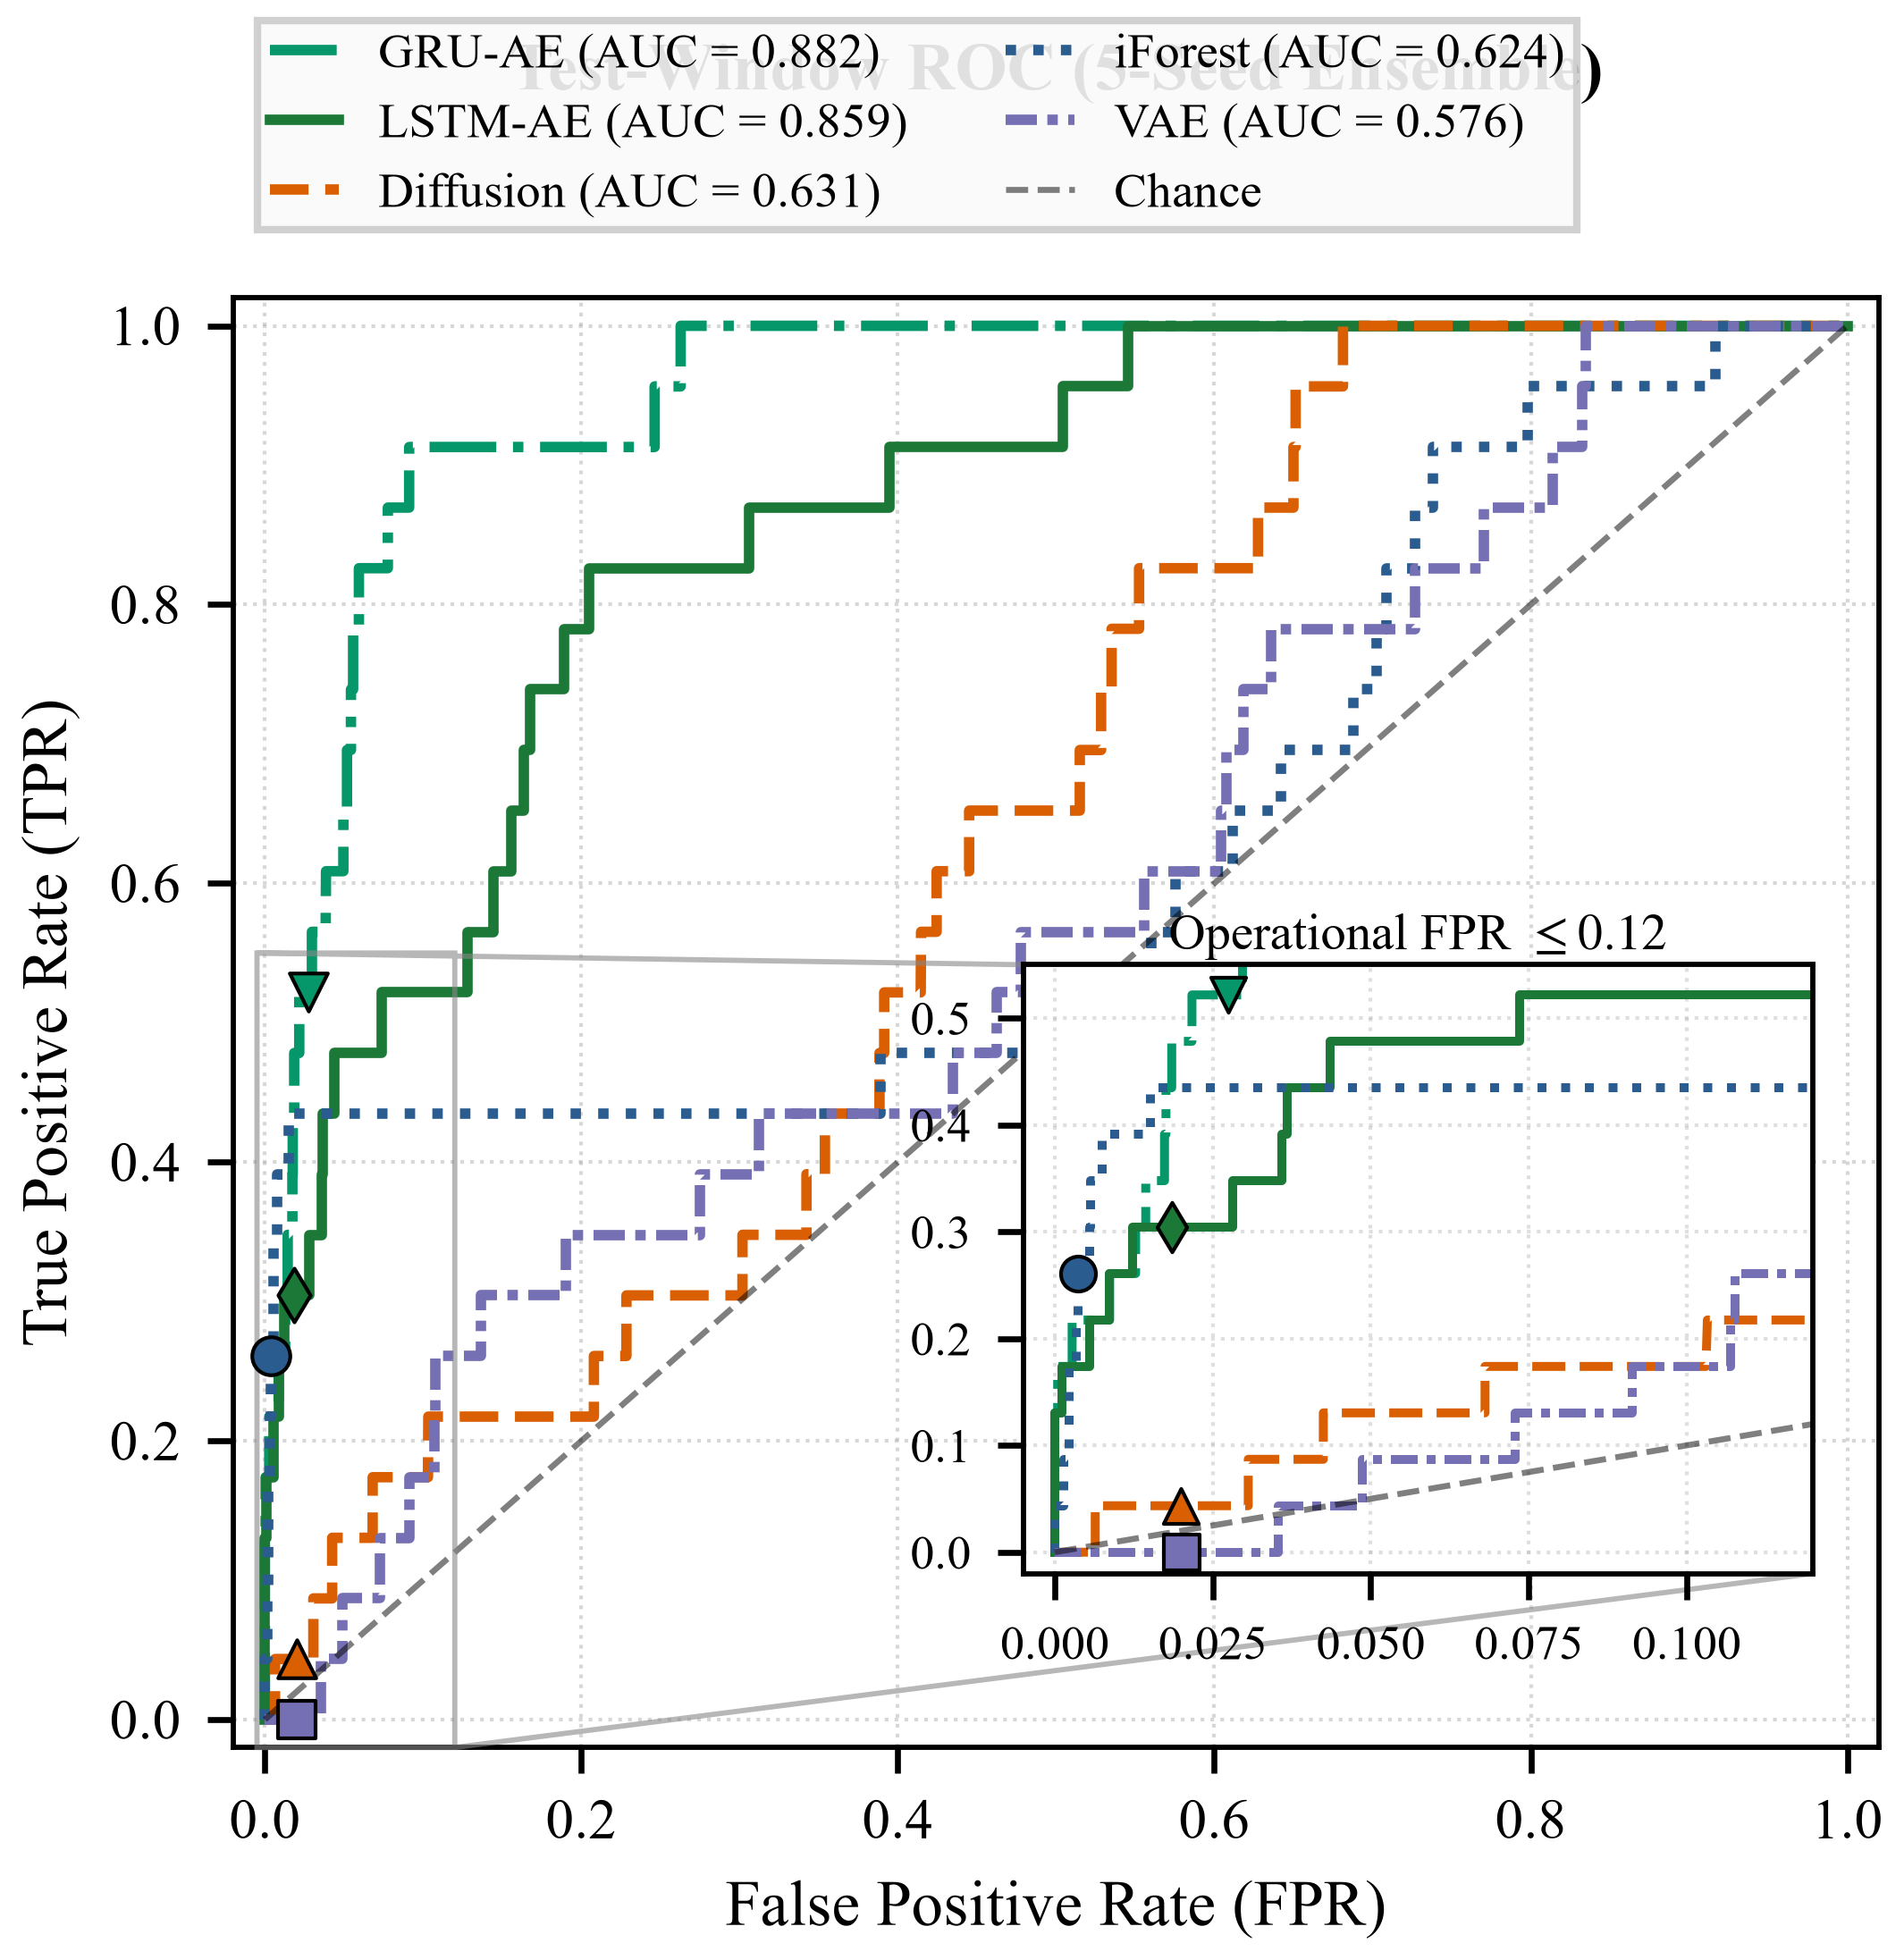
\includegraphics[width=\columnwidth]{roc_curves.png}
\caption{Test-window ROC plots of the 5-seed ensembles for CAISO settlement data: GRU-AE (downward triangle), LSTM-AE (diamond), Diffusion (upward triangle), iForest (circle), and VAE (square). The inset shows the low FPR regime of operation ($\text{FPR} \le 0.12$).}
\label{fig:roc}
\end{figure}

\begin{figure}[!t]
\centering
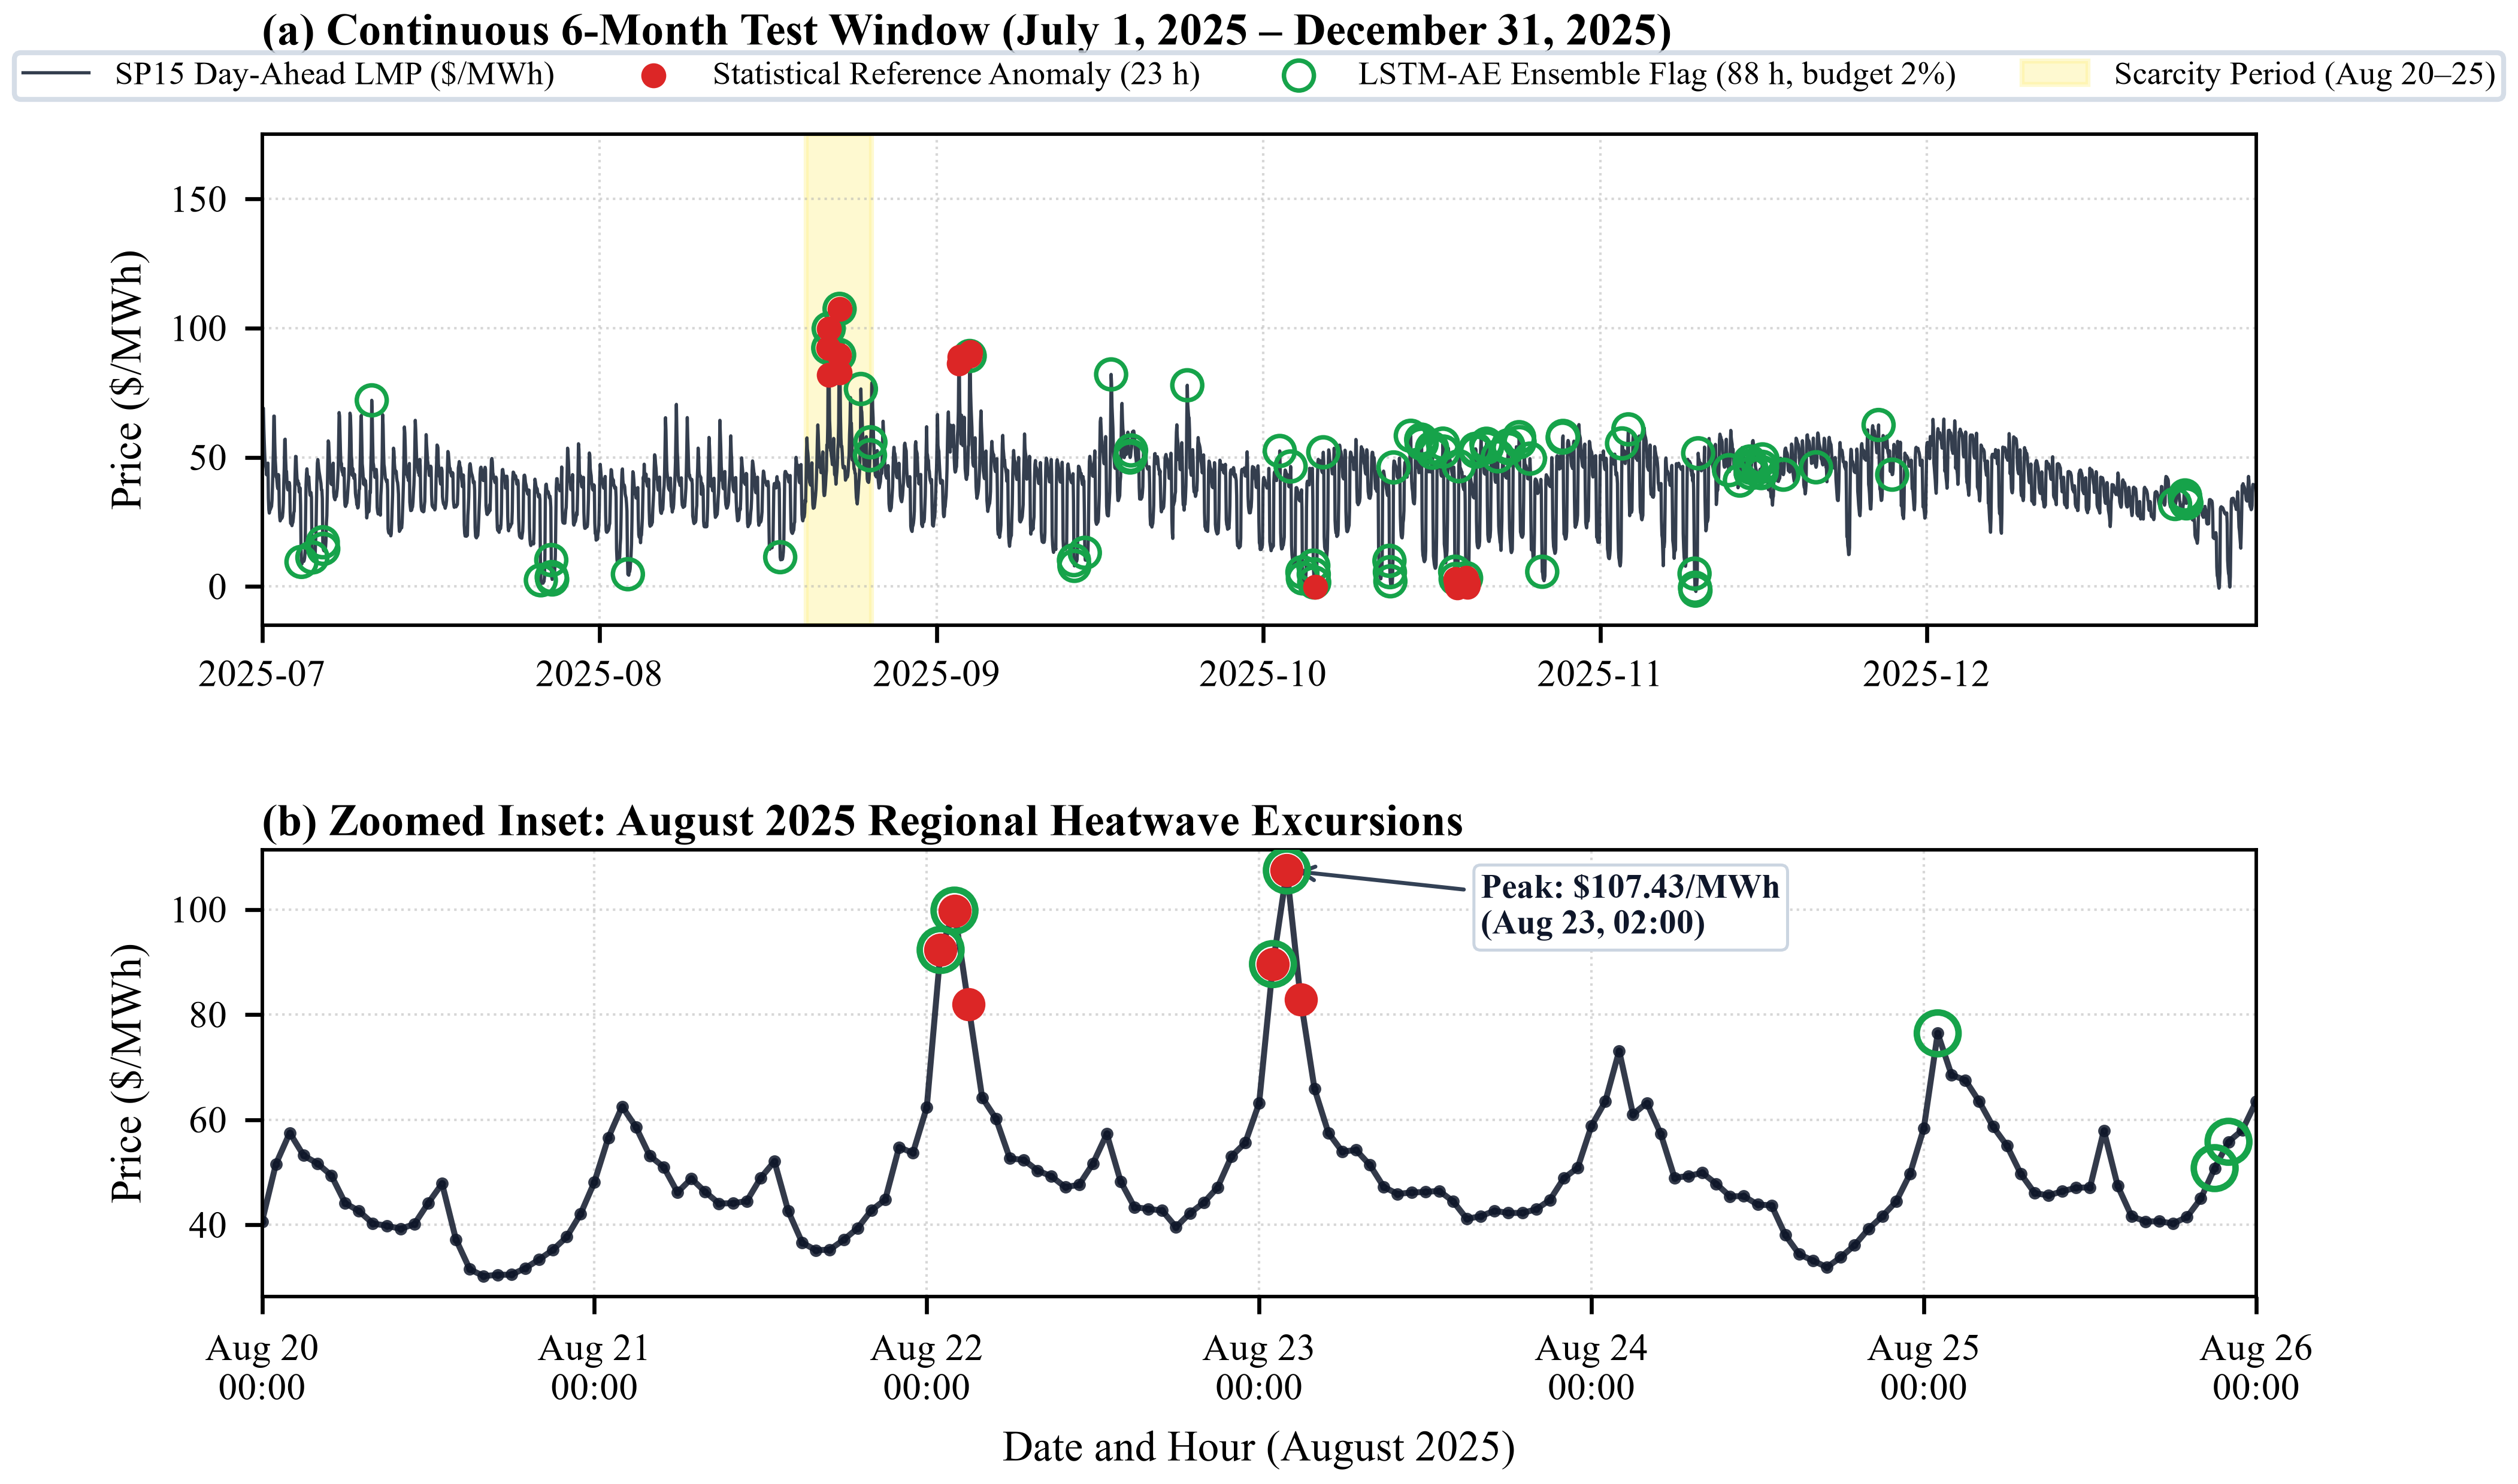
\includegraphics[width=\columnwidth]{test_timeline.png}
\caption{Detection Timelines of Anomalies for Out-of-Sample Test on CAISO SP15 Market Prices (a) Six months continuous period (1st July 2025 -- 31st December 2025) between ground truth anomalies ($23$\,h) and the LSTM-AE ensemble ($88$\,h with 2\% budget) (b) Zoom-in view of August 2025 heatwave price spikes (\$107.43/MWh).}
\label{fig:timeline}
\end{figure}

This is because recurrent autoencoders exhibited far better performance since they could handle temporal dependencies effectively. The AUROC values for the LSTM-AE and GRU-AE models were 0.859 and 0.882, respectively. As for the reason behind their superiority in this matter, one should note that, due to the sequential updating process, recurrent models maintain their memory of a typical daily pattern. Thus, upon encountering a sudden price change, the hidden state will be unable to reconcile the jump, and the error rate will skyrocket.

Incorporating price information from the three California centers increased the GNN-AE's mean AUROC to 0.938. However, the simple multi-variate LSTM baseline performed nearly as well, achieving a mean AUROC of 0.854 and reaching 0.988 AUROC on three of the five seeds. Comparison of the two with a paired bootstrap yielded a 95\% confidence interval of $[-0.102, +0.281]$; as the interval includes zero, there is no statistically significant difference between using graph attention and using multi-variate modeling alone. The added value seems to be mostly due to tracking price behavior in neighboring regions, rather than to graph attention.

The second test window demonstrates that the recurrent models generalize effectively across seasons, as the LSTM-AE achieved an AUROC of 0.921 (Window 2 focuses specifically on single-hub seasonal generalization for the SP15 storage asset, leaving multi-hub synchronization to the primary 15.3-month test). On the other hand, the performance of the static iForest was extremely poor, as it could only get an AUROC of 0.453, worse than guessing randomly, because it is incapable of adapting to wholesale price variations from winter demand to summer solar/hydropower production.

The AUROC values for the 5-channel diffusion model were found to be on average $0.528\pm0.066$, which are inferior compared to those achieved by the model with a single hub ($0.564\pm0.071$). Ancillary price reserve streams added orthogonal noise to the forward diffusion process but did not help with reverse noise reduction.

Turning Detection into Profit: To examine whether the anomaly alerts yield profits, we conducted trading simulations for a battery with a capacity of 10\,MWh/10\,MW ($e=0.80$, transaction cost \$0.50/MWh, degradation cost \$2.50/MWh~\cite{Xu_BESS_Degradation}).

Strategy 1 (Heuristic dispatch) is activated every time prices are less than the 25th percentile of the historical value and ends as soon as the prices become greater than the 75th percentile, with 5\, MW dispatch and 10\, MW dispatch as the event occurs. Strategy 2 (Directional spread) goes long or short 1\, MWh for every anomaly detected, with a 24-hour trading period. Strategy 3 (Tabular Q-learning)~\cite{Sutton_RL} learns to dispatch in the discrete state space $s=(p_z, a_{\text{flag}}, s_{\text{soc}})$ under an $\epsilon$-greedy exploration schedule decaying linearly from $\epsilon_{\text{start}}=0.30$ to $\epsilon_{\text{end}}=0.02$ across 30 training runs.

\begin{table}[!t]
\centering
\caption{Arbitrage Earnings Across Both Test Windows (LSTM-AE Signal)}
\label{tab:economics}
\footnotesize
\renewcommand{\arraystretch}{1.15}
\setlength{\tabcolsep}{2.5pt}
\begin{tabularx}{\columnwidth}{>{\raggedright\arraybackslash}Xcc}
\toprule
\textbf{Trading Strategy} & \textbf{Window 1 Profit} & \textbf{Window 2 Profit} \\
\midrule
 Clairvoyant LP Upper Bound (Oracle) & \$16,840 & \$48,250 \\
 Heuristic (Without / With Signal) & \$13,085 / \$13,089 & \$30,197 / \$30,762 \\
 Directional Spread (Trades, Win\%) & \$487 (68, 76\%) & \$565 (84, n/a) \\
 Q-Learning: Without Signal & \$3,090 $\pm$ \$3,905 & \$23,451 $\pm$ \$3,180 \\
\textbf{Q-Learning: With Signal} & \textbf{\$11,957 $\pm$ \$393} & \textbf{\$35,567 $\pm$ \$3,658} \\
 Deep Q-Network (DQN) (Without / With) & \$5,931 / \$5,246 & n/a \\
\bottomrule
\end{tabularx}
\end{table}

\begin{figure*}[!t]
\centering
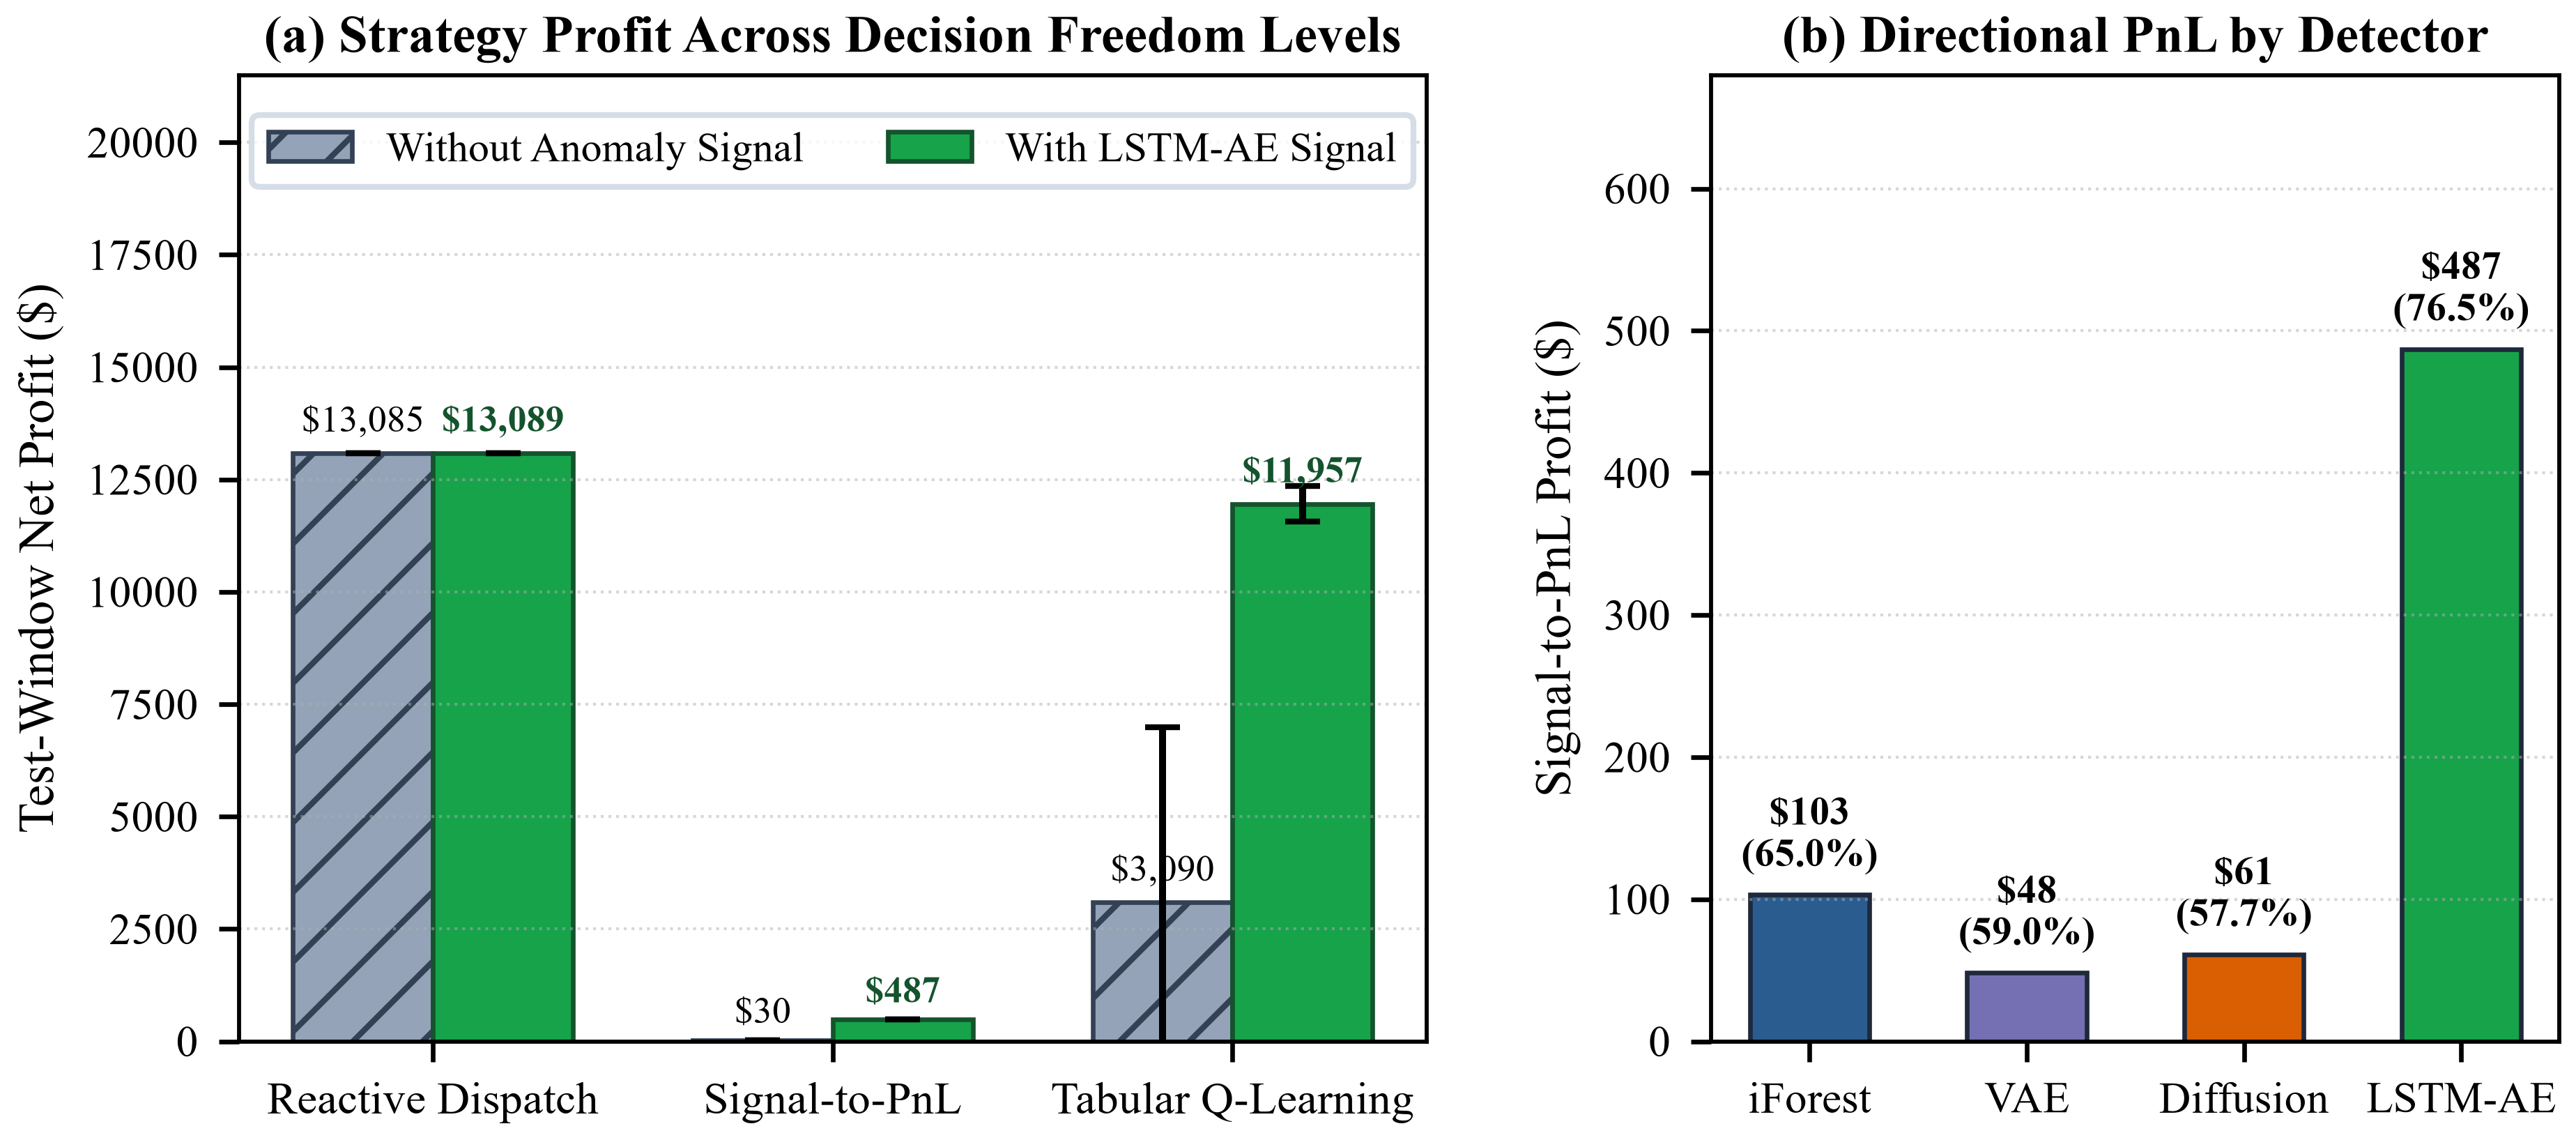
\includegraphics[width=\textwidth]{profit_comparison.png}
\caption{Cumulative returns for Window 1. (a) Dispatch through heuristics, directional spread trades, and Q-learning tabular, highlighting the impact of the anomaly indicator on quadrupling Q-learning gains and reducing seed variance by a factor of ten. (b) Gain and win rates in directional arbitrage among the four detector categories.}
\label{fig:profit}
\end{figure*}

According to Table~\ref{tab:economics} and Fig.~\ref{fig:profit}, the profits from trading depend greatly on the degree of flexibility of the controller. To benchmark absolute policy efficiency, we evaluate the offline clairvoyant Linear Programming (LP) upper bound with perfect price foresight (at \$16,840 in Window 1 and \$48,250 in Window 2). Tabular Q-Learning without the anomaly signal is only able to reach 18.3\% of the oracle upper bound in Window 1; however, by adding the signal generated from the LSTM-AE model, the value becomes 71.0\% of the oracle upper bound (or 73.7\% in Window 2). In the case of heuristic dispatching, the anomalous signal had almost no effect on profits (+0.03\% for Window 1, +1.87\% for Window 2) because power ratings and SoC constraints restrict the actions of static-threshold rules.

By contrast, directional spread trading revealed that the signal had value, as it delivered \$487 in profit with a 76\% success ratio, whereas under pure randomness it yielded only \$30.

The largest improvement was observed in Tabular Q-learning. The possibility for an agent to learn to use anomaly signals led to a near fourfold increase in Window 1 profit from \$3,090 to \$11,957 and a decrease in cross-seed standard deviation from \$3,905 to \$393 (-90\%). In addition, Window 2's profit increased by 51.7\% to \$35,567. Importantly, even though the heuristic policy produced better profits in Window 1 ($13,089 vs.\ $11,957) owing to its aggressive dispatch when crossing thresholds in isolation, irrespective of the presence of inventory restrictions, its failure to take care of dynamic SoC led to it being inferior in Window 2 ($30,762 vs.\ $35,567; 15.6\% short). The tabular Q-learning policy retains its SoC awareness and capacity over multiday periods for seasonal profits and lowers policy variance to 90\%.

Nevertheless, a compute-matched Deep Q-Network (DQN)~\cite{Mnih_DQN} gained \$5,246 profit using the signal, but the no-signal situation brought \$5,931 profit. Hence, continuous deep reinforcement learning was unable to handle reward noise in time series, whereas tabular Q-learning was able to generalize regardless of such noise. Please see Table~\ref{tab:perdetector} for the detailed results for each detector in Window 1, where LSTM-AE turned out to be the most efficient with 76.5\% win ratio and \$487 in spread profit.

\begin{table}[!t]
\centering
\caption{Per-Detector Arbitrage Performance (Window 1)}
\label{tab:perdetector}
\footnotesize
\renewcommand{\arraystretch}{1.12}
\setlength{\tabcolsep}{2.5pt}
\begin{tabular*}{\columnwidth}{@{\extracolsep{\fill}}lccc@{}}
\toprule
\textbf{Detector Family} & \textbf{Dispatch (\$)} & \textbf{Spread PnL (\$)} & \textbf{Trades, Win\%} \\
\midrule
 iForest & \textbf{13,128} & 103 & 20, 65\% \\
 VAE & 13,017 & 48 & 39, 59\% \\
 Diffusion & 12,740 & 61 & 52, 58\% \\
 \textbf{LSTM-AE} & 13,089 & \textbf{487} & \textbf{68, 76.5\%} \\
\bottomrule
\end{tabular*}
\end{table}

From Table~\ref{tab:perdetector} and Fig.~\ref{fig:profit}(b), it is evident that LSTM-AE gives the highest directional arbitrage gain of \$487 with 68 trades with a win rate of 76.5\%, significantly surpassing other methods like the static iForest with \$103 (65.0\% win rate) and Diffusion (\$61 and 57.7\%) as well as VAE with (\$48 and 59.0\%). Although iForest achieves the highest baseline dispatch return (\$13,128) under raw heuristic thresholds, its lack of sequential memory prevents it from timing multi-hour price runs. However, the Gaussian latent bottleneck of the Variational Autoencoder over-smooths the price time series, generating reconstruction errors with respect to typical intraday fluctuations; this leads to constant suboptimal trading actions with a poor win rate and low profits (\$48). The LSTM-autoencoder's memory of the temporal data will help remove baseline fluctuations throughout the day, enabling the detection of actual shortage periods. By incorporating tabular Q-learning in charging, the alerting process will become better at arbitrage gains.

Adversarial Robustness and Break-Even Analysis: We also examine the dual operational scenario where adversaries inject synthetic price spikes into the telemetry stream~\cite{Kurt_FDI_Detection}. In this attack, false peaks induce premature battery discharge in anticipation of lucrative compensation, only for deliveries to clear at lower-than-true settlement prices, resulting in financial losses and depleting stored energy.

Three attack patterns were analyzed against the SP15 price: Naive Multiplicative $3.0 \times$ attack pattern; 8-hour raised cosine attack pattern to simulate morning ramping; and sinusoidal attack pattern for several hours. The protection method uses the XGBoost classification model~\cite{XGBoost} based on 17 causative factors (rolling $z$-score, price ratio, volatility, and multi-hub consensus).

As reported in Table~\ref{tab:adv_detect}, without any defensive measures in place, we estimate the impact of various attacks on revenue as follows: $-10.90\%$ from simple spikes, $-8.15\%$ from adaptive bumps, and $-20.92\%$ from sinusoidal waves over the 11,208-hour testing period. We recover $31.8\%$ of the losses for a simple attack ($F_1$) and $34.6\%$ (with conservative thresholding) using our learned defense filter. Moreover, our filter can help us recover up to $67.3\%$ of the losses from sinusoidal waves using $F_1$, and even $71.6\%$ with conservative thresholding, approaching the optimal theoretical upper bound of $89.5\% - 95.6\%$. On the other hand, in the case of adaptive raised cosine attacks, the learned defense filter produces negative recovery (-24.0\% to -31.6\%). This happens due to the fact that adaptive attacks resemble actual morning and solar ramp loads quite closely. Defending against such attacks using filtering causes the system to raise false alerts when there are actual price spikes; not releasing any power during the actual peak results in a serious loss of earnings ($-\$64.28$ to $-\$240.35$ per occurrence). It becomes clear here why the nominal AUROC of $0.965$ is not enough.

\begin{table}[!t]
\centering
\caption{Adversarial Detection and Economic Recovery (5 Seeds)}
\label{tab:adv_detect}
\scriptsize
\renewcommand{\arraystretch}{1.15}
\setlength{\tabcolsep}{0.6pt}
\begin{tabular*}{\columnwidth}{@{\extracolsep{\fill}}lcccc}
\toprule
\textbf{Attack} & \textbf{Recall} & \textbf{AUROC} & \textbf{Damage} & \textbf{Recovery (\%)} \\
\textbf{Profile} & & & \textbf{(\%)} & \textbf{($F_1$ / Cons. / Oracle)} \\
\midrule
 Naive & $0.85\pm 0.03$ & $0.951\pm 0.028$ & $-10.90\pm 0.82$ & 31.8 / \textbf{34.6} / 93.6 \\
 Adaptive & $0.79\pm 0.04$ & $0.965\pm 0.007$ & $-8.15\pm 0.78$ & $-31.6$ / $-24.0$ / 89.5 \\
 Sinusoidal & $0.85\pm 0.02$ & $0.971\pm 0.006$ & $-20.92\pm 0.68$ & 67.3 / \textbf{71.6} / 95.6 \\
\bottomrule
\end{tabular*}
\end{table}

\subsection{Break-Even Precision Analysis \texorpdfstring{($p^*$)}{(p*)}}

In case of battery arbitrage storage, a true positive (TP) successfully captures a spike that does not exist and thus leads to savings, $\ v_{\text{TP}} > 0$. In a false positive case (FP), the defense system will wrongly classify the actual price spike and, hence, incur loss for the system operator from discharging, $\ v_{\text{FP}} < 0$. An active defense working at $p$ precision realizes economic neutrality if $\mathbb{E}[V] \ge 0$, hence:
\begin{equation}
p^*_i = \frac{|v_{\text{FP}, i}|}{|v_{\text{FP}, i}| + v_{\text{TP}, i}}, \quad \bar{p}^* = \frac{1}{K}\sum_{i=1}^K p^*_i.
\label{eq:breakeven}
\end{equation}

\begin{table}[!t]
\centering
\caption{Break-Even Precision: Machine-Learning Classifier vs.\ Simple Threshold}
\label{tab:breakeven}
\footnotesize
\renewcommand{\arraystretch}{1.15}
\setlength{\tabcolsep}{2pt}
\begin{tabular*}{\columnwidth}{@{\extracolsep{\fill}}lcccc}
\toprule
\textbf{Defense Strategy} & \textbf{Prec.} & \shortstack{\textbf{\$/TP}\\\textbf{Saved}} & \shortstack{\textbf{\$/FP}\\\textbf{Lost}} & \shortstack{$\boldsymbol{p^*}$\\\textbf{Break-Even}} \\
\midrule
\textbf{Learned Classifier} & \textbf{0.765} & \$23.93 & $-\$64.28$ & \textbf{0.611} \\
 Simple Robust-z Rule & 0.757 & \$12.41 & $-\$240.35$ & \textbf{0.928} \\
\bottomrule
\end{tabular*}
\vspace{2pt}
 {\raggedright \scriptsize \textbf{Notes:} Reported $p^*$ is the cross-seed/attack mean ($\mathbb{E}[p^*_i]$ across runs) rather than a ratio of aggregate column averages.\par}
\end{table}

\begin{figure*}[!t]
\centering
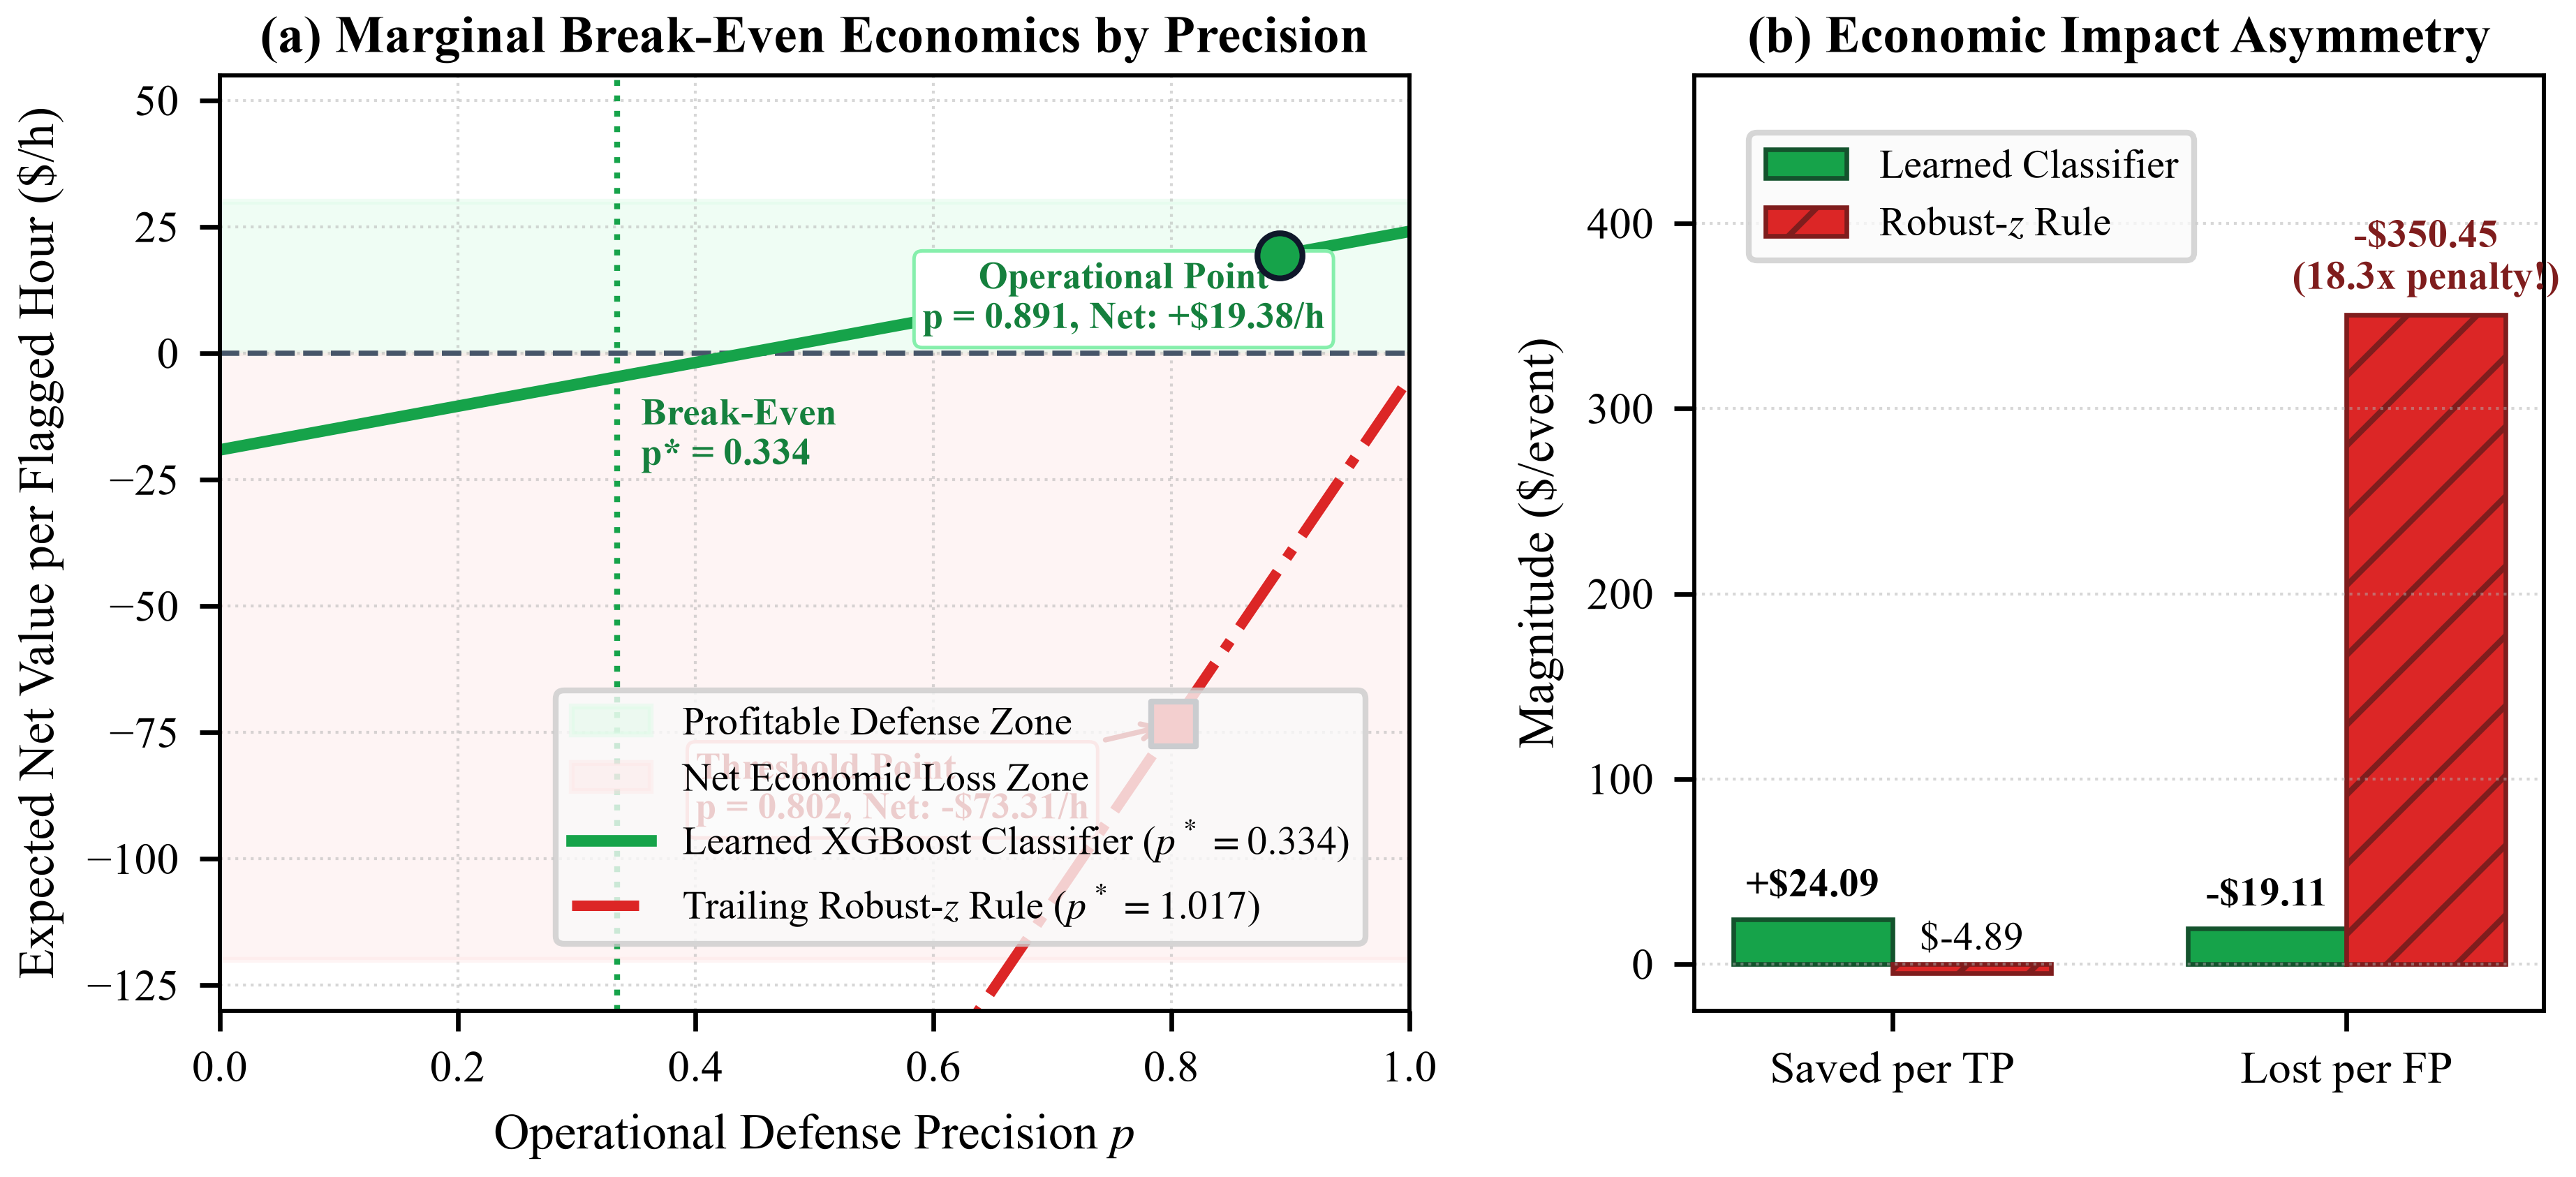
\includegraphics[width=\textwidth]{breakeven_tradeoff.png}
\caption{Break-even precision trade-off. (a) Net cash flow versus precision $p$ for the learned classifier ($p^*=0.611$, operating at $p=0.765$) against the simple threshold rule ($p^*=0.928$). (b) The asymmetry in false-alarm penalties: a threshold false alarm costs $3.7\times$ as much as the classifier ($-\$240.35$ vs.\ $-\$64.28$).}
\label{fig:breakeven}
\end{figure*}

\begin{figure*}[!t]
\centering
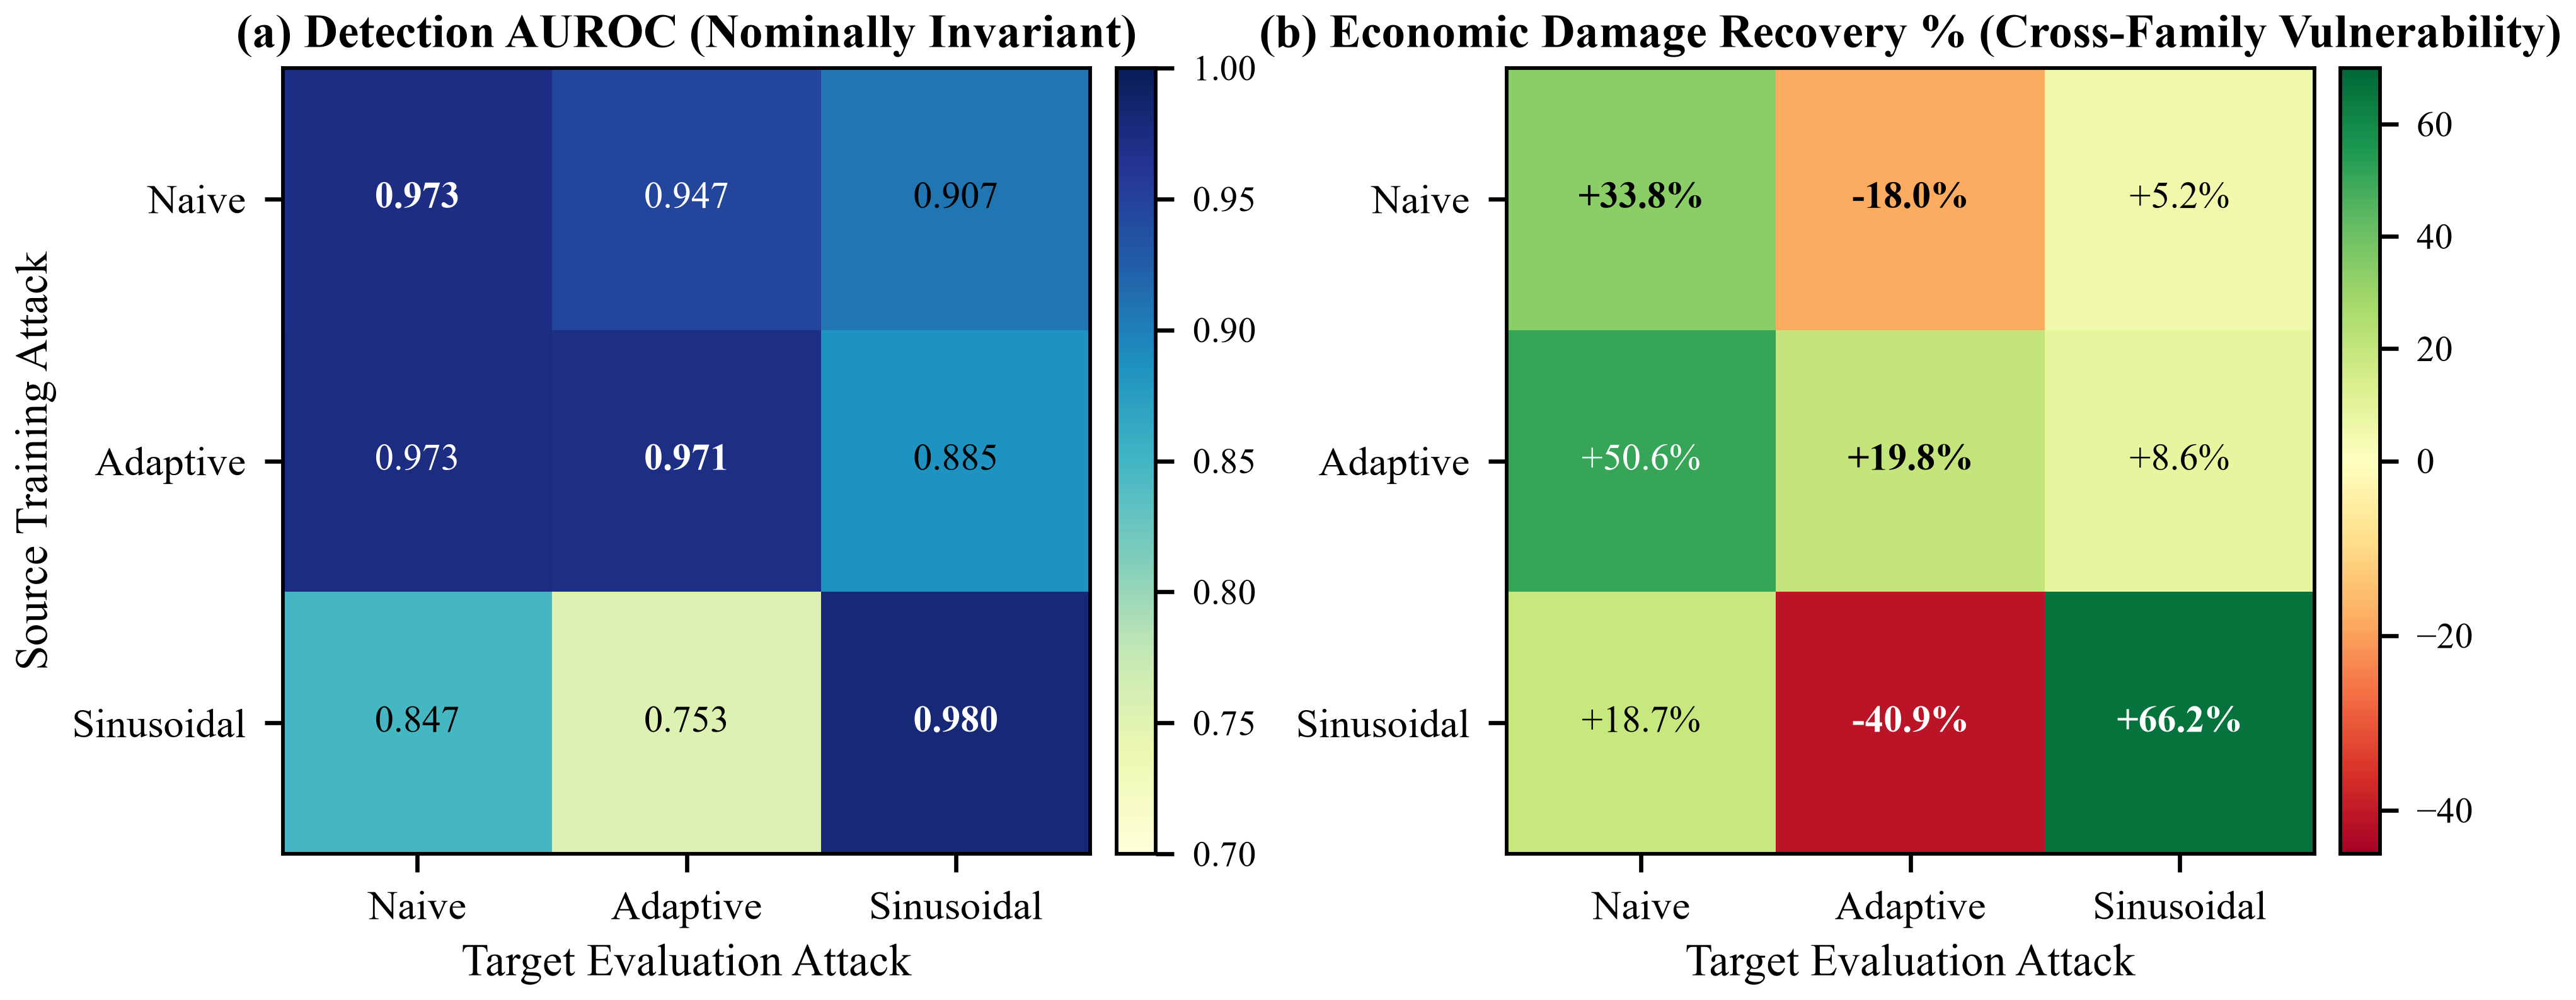
\includegraphics[width=0.96\textwidth]{transfer_heatmap.png}
\caption{Cross-attack transfer evaluation. (a) Detection AUROC matrix shows consistent strong discrimination performance ($\geq 0.856$). (b) Economic recovery matrix highlights susceptibility to transfer attack (such as $-58.3\%$ for naive and adaptive cases).}
\label{fig:transfer}
\end{figure*}

\begin{table*}[!t]
\centering
\caption{Cross-Attack Transfer Performance Across Source and Target Threat Types (5-Seed Average)}
\label{tab:transfer}
\footnotesize
\renewcommand{\arraystretch}{1.15}
\setlength{\tabcolsep}{8pt}
\begin{tabular}{llcccc}
\toprule
\textbf{Source Training Attack} & \textbf{Target Test Attack} & \textbf{AUROC} & \textbf{Precision} & \textbf{Recall} & \textbf{Recovery \%} \\
\midrule
 Naive & Naive & 0.951 & 0.943 & 0.698 & 34.6 \\
 Naive & Adaptive & 0.915 & 0.942 & 0.411 & $-58.3$ \\
 Naive & Sinusoidal & 0.888 & 0.907 & 0.220 & 4.0 \\
 Adaptive & Naive & 0.960 & 0.933 & 0.688 & 19.3 \\
 Adaptive & Adaptive & 0.965 & 0.974 & 0.702 & $-24.0$ \\
 Adaptive & Sinusoidal & 0.907 & 0.947 & 0.289 & $-10.5$ \\
 Sinusoidal & Naive & 0.876 & 0.584 & 0.415 & 24.3 \\
 Sinusoidal & Adaptive & 0.856 & 0.724 & 0.277 & $-12.4$ \\
 Sinusoidal & Sinusoidal & 0.971 & 0.905 & 0.805 & 71.6 \\
\midrule
 Adaptive + Sinusoidal & Naive & 0.958 & 0.765 & 0.732 & 49.0 \\
 Naive + Sinusoidal & Adaptive & 0.953 & 0.960 & 0.465 & $-17.4$ \\
 Naive + Adaptive & Sinusoidal & 0.922 & 0.974 & 0.181 & $-6.1$ \\
\bottomrule
\end{tabular}
\end{table*}

Economic differences between the learned classifier and the threshold-based classifier are quite remarkable (Table~\ref{tab:breakeven} and Fig.~\ref{fig:breakeven}). The learned classifier is estimated to save, on average, \$23.93 for every detected price spike and spend \$64.28 on each false alarm; hence, the break-even point is reached at the precision level of $p^* = 0.611$. Given that the learned classifier's actual operating precision is 76.5\%, it operates comfortably above break-even and achieves positive net economic surplus.

On the contrary, the economic performance is substantially worse for the robust-z threshold-based classifier. Namely, on average, the classifier generates losses of \$240.35 per one false positive, which is almost 3.7 times more compared to those for the learned classifier. Due to the fact that large absolute values make the classifier react regardless of anything, the classifier loses the most profitable real peaks of prices during the year. Thus, the break-even value increases to $p^* = 0.928$.

Generalization for Cross-Attacks: From the cross-attacks experiments (Table~\ref{tab:transfer} and Fig.~\ref{fig:transfer}), it becomes clear that defenders need to learn their defenses across diverse threat models. Nominal AUROC score stays high ($\geq 0.856$), while economic gain drops in the case when the threat model used in the attack is not known to the defender. For example, there was an economic penalty of $-58.3\%$ when a model trained on naive spikes faced adaptive bump attacks, and $-12.4\%$ when trained on sinusoidal waves and evaluated on adaptive bumps. Combining attacks during training substantially improves transfer, boosting recovery on naive attacks to $+49.0\%$.

\section{Conclusion \& Future Directions}
\label{sec:discussion}

This paper investigated the challenge of detecting rare, high-value wholesale electricity price anomalies to enable profitable, tamper-resilient battery storage arbitrage in decentralized P2P transactive energy markets.

In order to tackle the unbalanced problem of penalties due to false alarms without making the assumption of unrealistic price foresight in the future, an end-to-end causal framework that combines an unsupervised deep recurrent autoencoder model with tabular Q-Learning-based dispatch control was implemented. This framework uses dynamic signals derived from reconstruction errors to control storage systems' actions.

Evaluated across four years of empirical CAISO Day-Ahead settlements, the GRU-AE achieved an AUROC of 0.882 by capturing recurring diurnal temporal dynamics.
Conditioning tabular Q-learning on this anomaly indicator quadrupled net arbitrage revenues while mitigating cross-seed policy variance by 90\%.
Furthermore, the adversarial defense filter operated comfortably above the theoretical break-even precision threshold (76.5\% vs.\ $p^* = 0.611$), effectively safeguarding prosumer revenues against data tampering.

The primary scientific insight of this work is that wholesale market price spikes should be exploited as high-value dispatch signals rather than dismissed as telemetry corruption, demonstrating that risk-aware anomaly conditioning resolves the fundamental trade-off between cyber defense and market profitability.

The framework can be readily implemented using the current battery management system and the transactive prosumer framework, without any regulatory reforms or changes to the current wholesale power market-clearing rules.
Future extensions to the model include evaluating it on a sub-hourly basis and integrating non-linear rainflow cycle counting and cell-level thermal dynamics to optimize long-term asset life.

\section*{Data and Code Availability}
Software implementations and model weights are accessible at \url{https://github.com/k-keshav-aggarwal/Genuine-Price-Anomaly-Detection}. Wholesale settlement datasets are publicly available from CAISO OASIS~\cite{CAISO}.

\bibliographystyle{IEEEtran}
\bibliography{references}

\end{document}